\documentclass[pdftex, twocolumn=true, parskip=half]{scrartcl}

%%% KOMA Script Optionen
\KOMAoptions{draft=on}

%%% Tech
\usepackage[final]{graphicx}
\usepackage[linktocpage]{hyperref}
\hypersetup{colorlinks=false, pdfborder={0 0 0}, pdftitle={}, pdfauthor={}}

%%% Typo
\usepackage[ngerman]{babel}
\usepackage[utf8]{inputenc}
\usepackage[T1]{fontenc}
\usepackage{helvet}
\usepackage{sansmath}
\usepackage{enumerate}
\usepackage{mdwlist}
\usepackage[activate=normal]{pdfcprot}
\usepackage[babel]{csquotes}
\usepackage{units}

%%% Math
\usepackage[sumlimits,intlimits,namelimits]{amsmath}
\usepackage{amssymb}
\usepackage{mathrsfs}
\usepackage{slashed}
\usepackage{bm}
\usepackage{bbm}
\usepackage{bbding}

\begin{document}
\title{PeP et al. Sommerakademie 2013}

\maketitle
\section{Forschung}
Seit der ersten Sommerakademie im Jahr 2011 ist die Darstellung der Dortmunder Forschungsschwerpunkte ein vorrangiges Ziel. Im Rahmen von Vorträgen von Alumni, Doktoranden und Masterstudenten werden wissenschaftliche Arbeiten präsentiert und passende Schwerpunkte im Studium vorgestellt: Physik interdisziplinär -- Abschlussarbeiten am MPI und am ISAS; Teilchenphysik -- Formfaktoren in der Flavourphysik, LHCb Ergebnisse, Neutrinophysik; Festkörperphysik -- Quantenpunkte und Quantencomputer.
%end of section
\section{Teilnehmervorträge}
Das Abendprogramm besteht traditionell aus Vorträgen der Teilnehmer. Vorgabe ist dabei eine unterhaltsame Darstellung eines Themas. Die Themengebiete ergeben sich dabei sowohl aus Problemen in Physik und Mathematik als auch aus den Hobbies der Teilnehmer. Eine Auswahl der Themen in diesem Jahr: Doping im Leistungssport, (Mathematische) Gleichdicke, Die Geschichte des Manga, E-Sports, Bildrauschen, Das Mikromort.
%end of section
\section{Projekte}
Erstmalig wurden in diesem Jahr gemeinsam mit den Teilnehmern Wochenprojekte entwickelt und durchgeführt. Die Projekte wurden protokolliert und für Zukünftige Veranstaltungen aufbereitet und ausgewertet.
\subsection{Astrofotografie}
Die Umgebung in den Bergen und der eindrucksvolle nächtliche Sternenhimmel boten eine ideale Vorraussetzung für den versuch Himmelsobjekte auf Fotos einzufangen. Mit einer einfachen Spiegelreflexkamera wurden verschiedene Objekte fotografiert und die grundsätzlichen physikalischen Probleme wie Belichtung, Bewegung der Objekte und Bildrauschen herausgearbeitet. Mit Hilfe eines Computerprogramms wurden aus einer Vielzahl von Langzeitbelichtungen gemittelte Bilder erstellt. Besonders eindrucksvoll ist dabei das Bild der Galaxie M101.
\begin{figure}[!h]
\centering
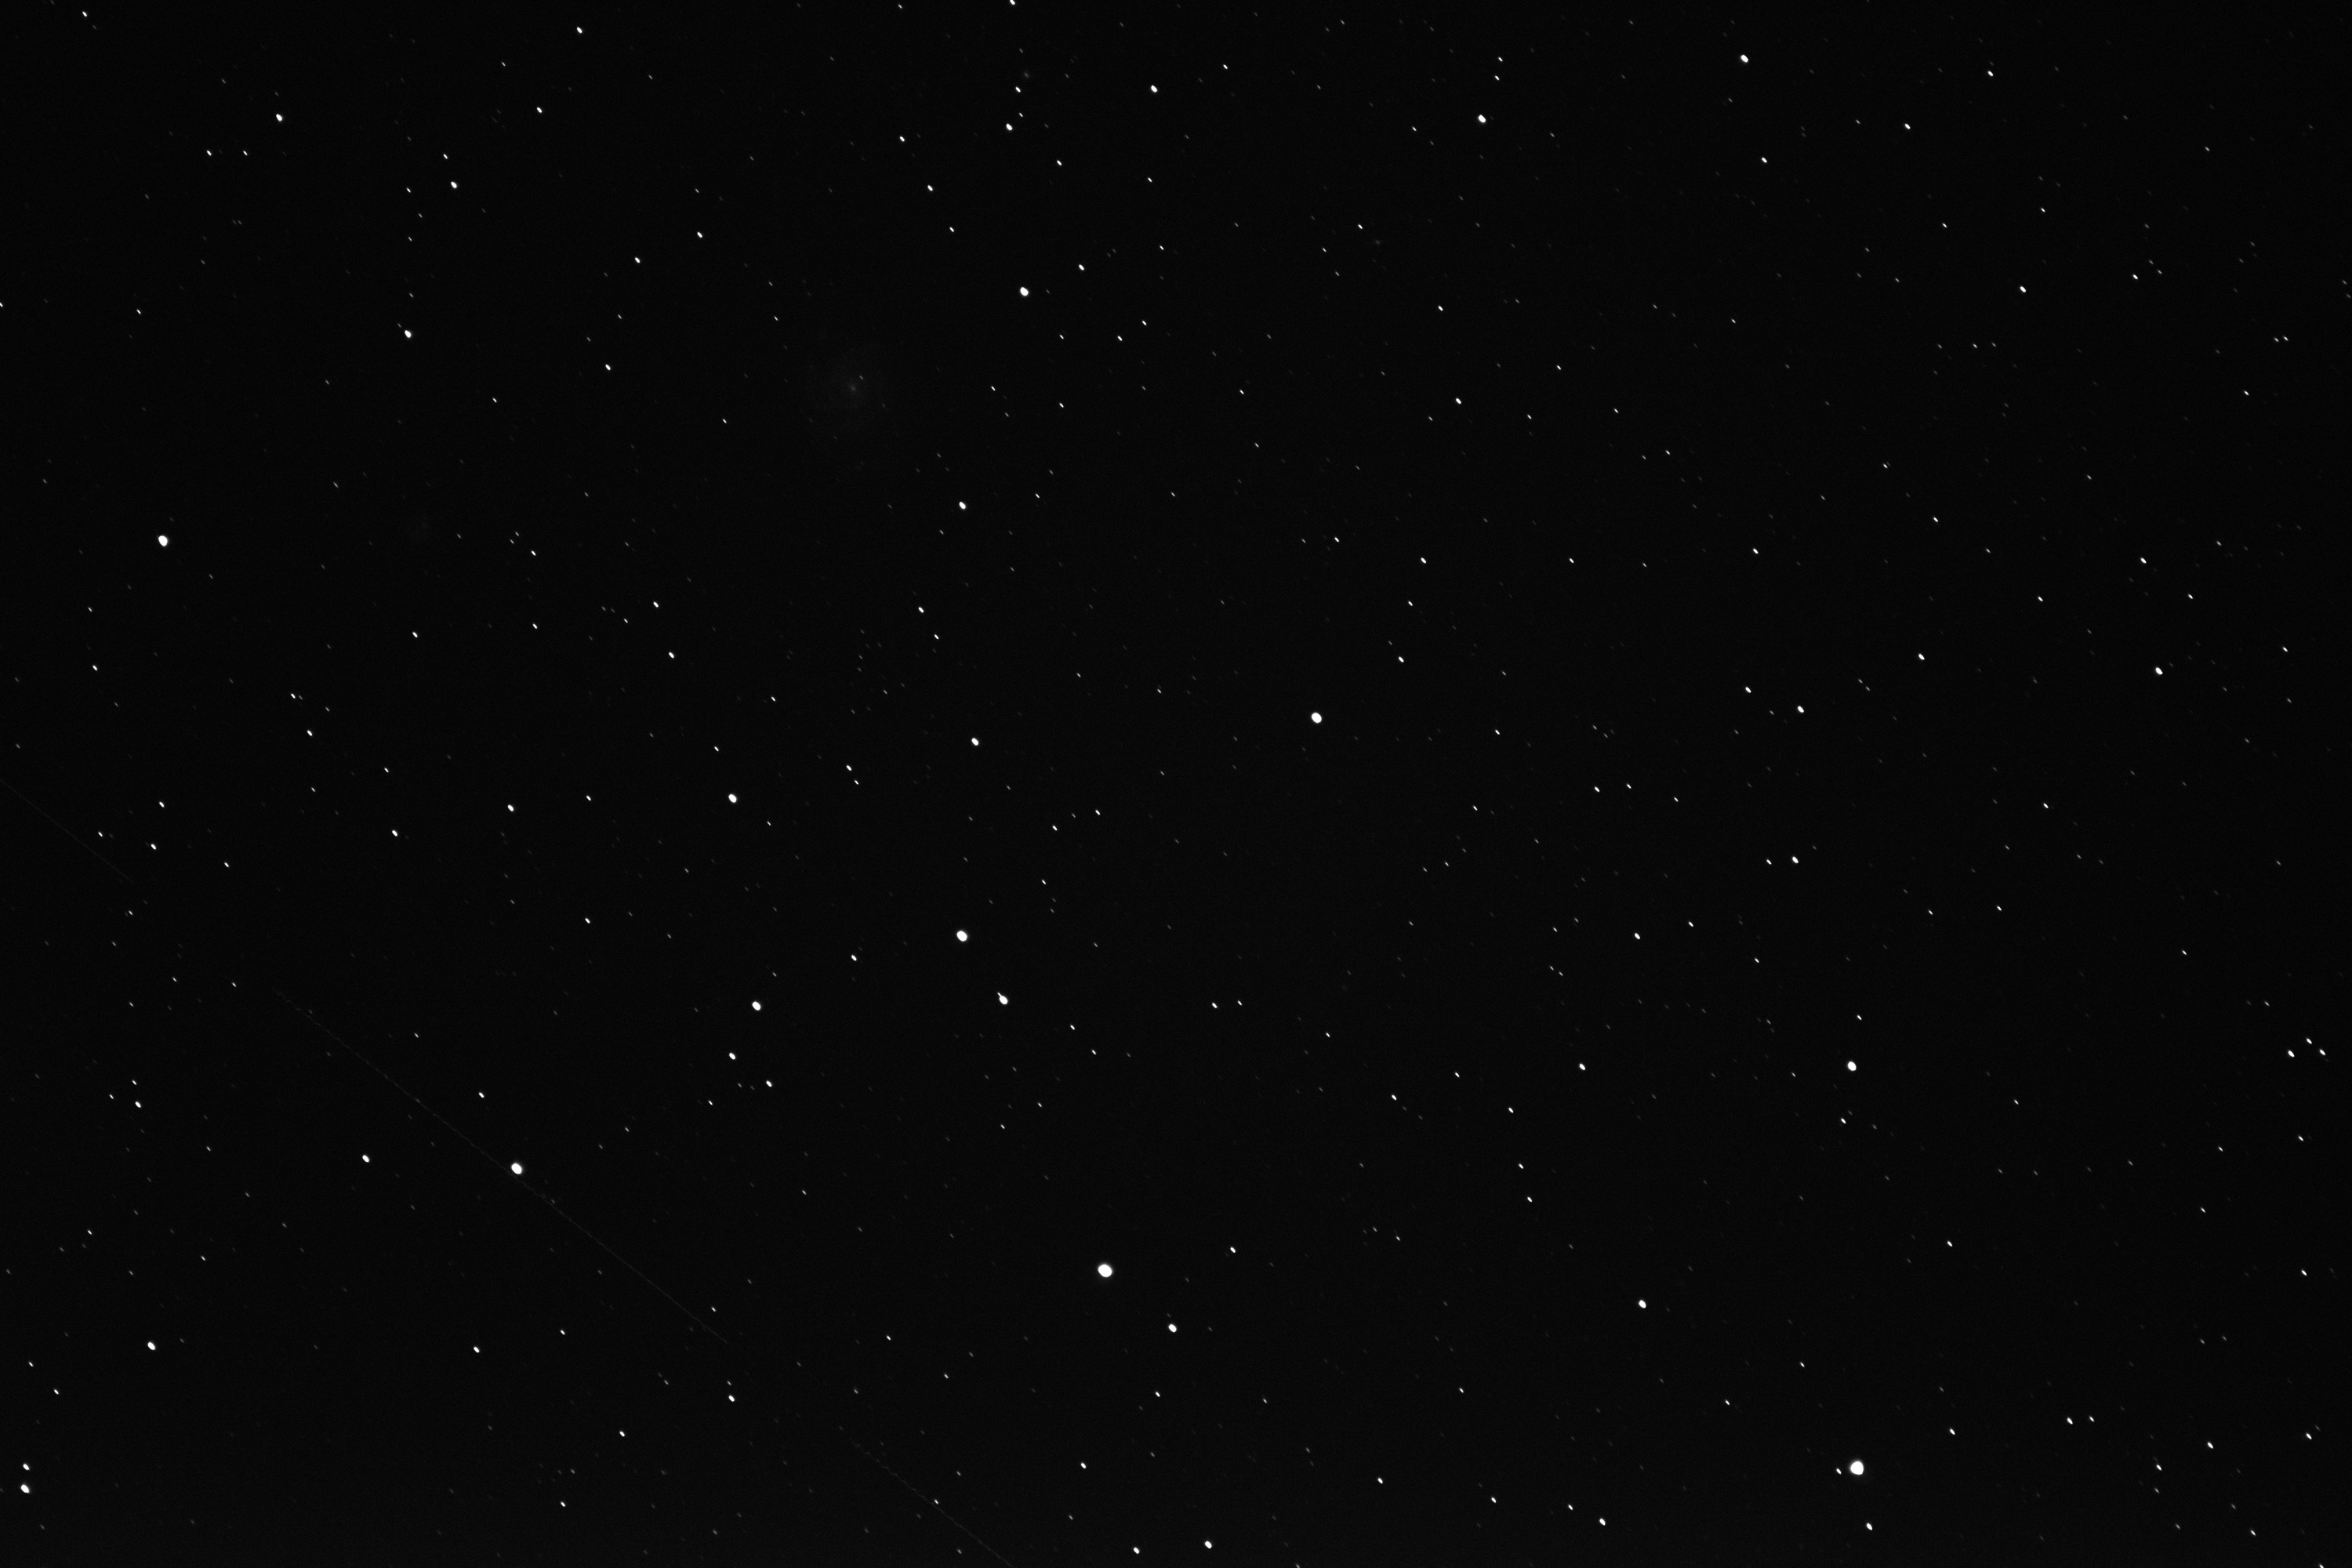
\includegraphics[width=0.45\textwidth]{figs/astro/m101_add_50.jpg}
\caption{Spiralgalaxie M101}
\end{figure}
%end of section
\subsection{Seismische Sensoren}
Zur Überwachung des Internationalen Teststoppvertrags für Nuklearwaffen werden seismische Sensoren eingesetzt. Im Rahmen dieses Projekts wurde eine elektronische Auslese auf Basis eines Arduinos implementiert und Software zur grafischen Darstellung der Messergebnisse entwickelt.

Das Projekt soll im nächsten Jahr weiterentwickelt werden. Durch die Verwendung von mehreren Sensoren soll eine Ortung von Fahrzeugen oder Tieren ermöglicht werden.
%end of section
\subsection{Wasserrakete}
Aus handelsüblichen Wasserflaschen und Materialien aus dem Baumarkt wurden Wasserraketen und eine Abschussvorrichtung gebaut. Damit wurden Messreihen zur Abhängigkeit der Steighöhe von Wasserdruck und Füllmenge erstellt.
\begin{figure}[!h]
\centering
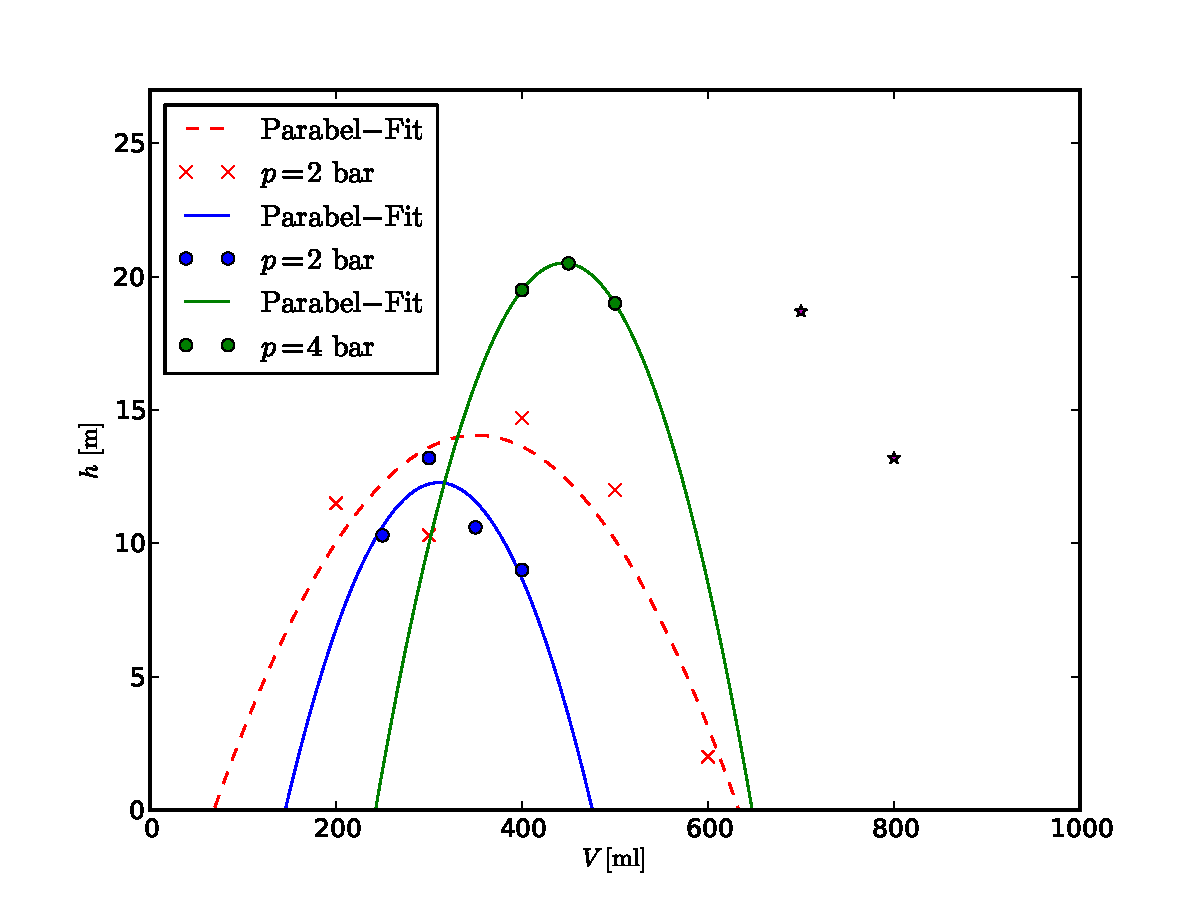
\includegraphics[width=0.45\textwidth]{figs/rakete/raketenplot.pdf}
\caption{Flughöhe der Rakete in Abhängikeit der Wasserfüllmenge}
\end{figure}
%end of section
\subsection{Solarofen}
Die Kraft der Sonne sollte ausgenutzt werden um einen Solarbetriebenen Ofen zu bauen. Nach der \textit{Sendung mit der Maus} sollen in einem Ofen aus zwei Pappkartons, schwarzer Farbe, einem Spiegel und etwas durchsichtiger Folie Temperaturen bis zu $\unit[140]{^oC}$ erreicht werden. Aufgrund fehlender Materialien für die Isolierung wurden diese Werte in diesem Jahr noch nicht erreicht.
%end of section
\section{Miteinander}
%end of section
Neben den physikalischen Inhalten der Sommerakademie ist die Förderung des Kontakts unter den Studierenden und der Aufbau eines Netzwerks, welches über die Zeit an der TU Dortmund bestand hat, ein wichtiges Ziel. Auch in diesem Jahr rundete eine Ausgiebige Wanderung auf die 2168 Meter hohe Mittagsspitze die Veranstaltung ab. In der Unterkunft versorgen sich die Teilnehmer selbst, so dass die täglichen Arbeiten fest ins gemeinsame Programm gehören.
\begin{figure}[!h]
\centering
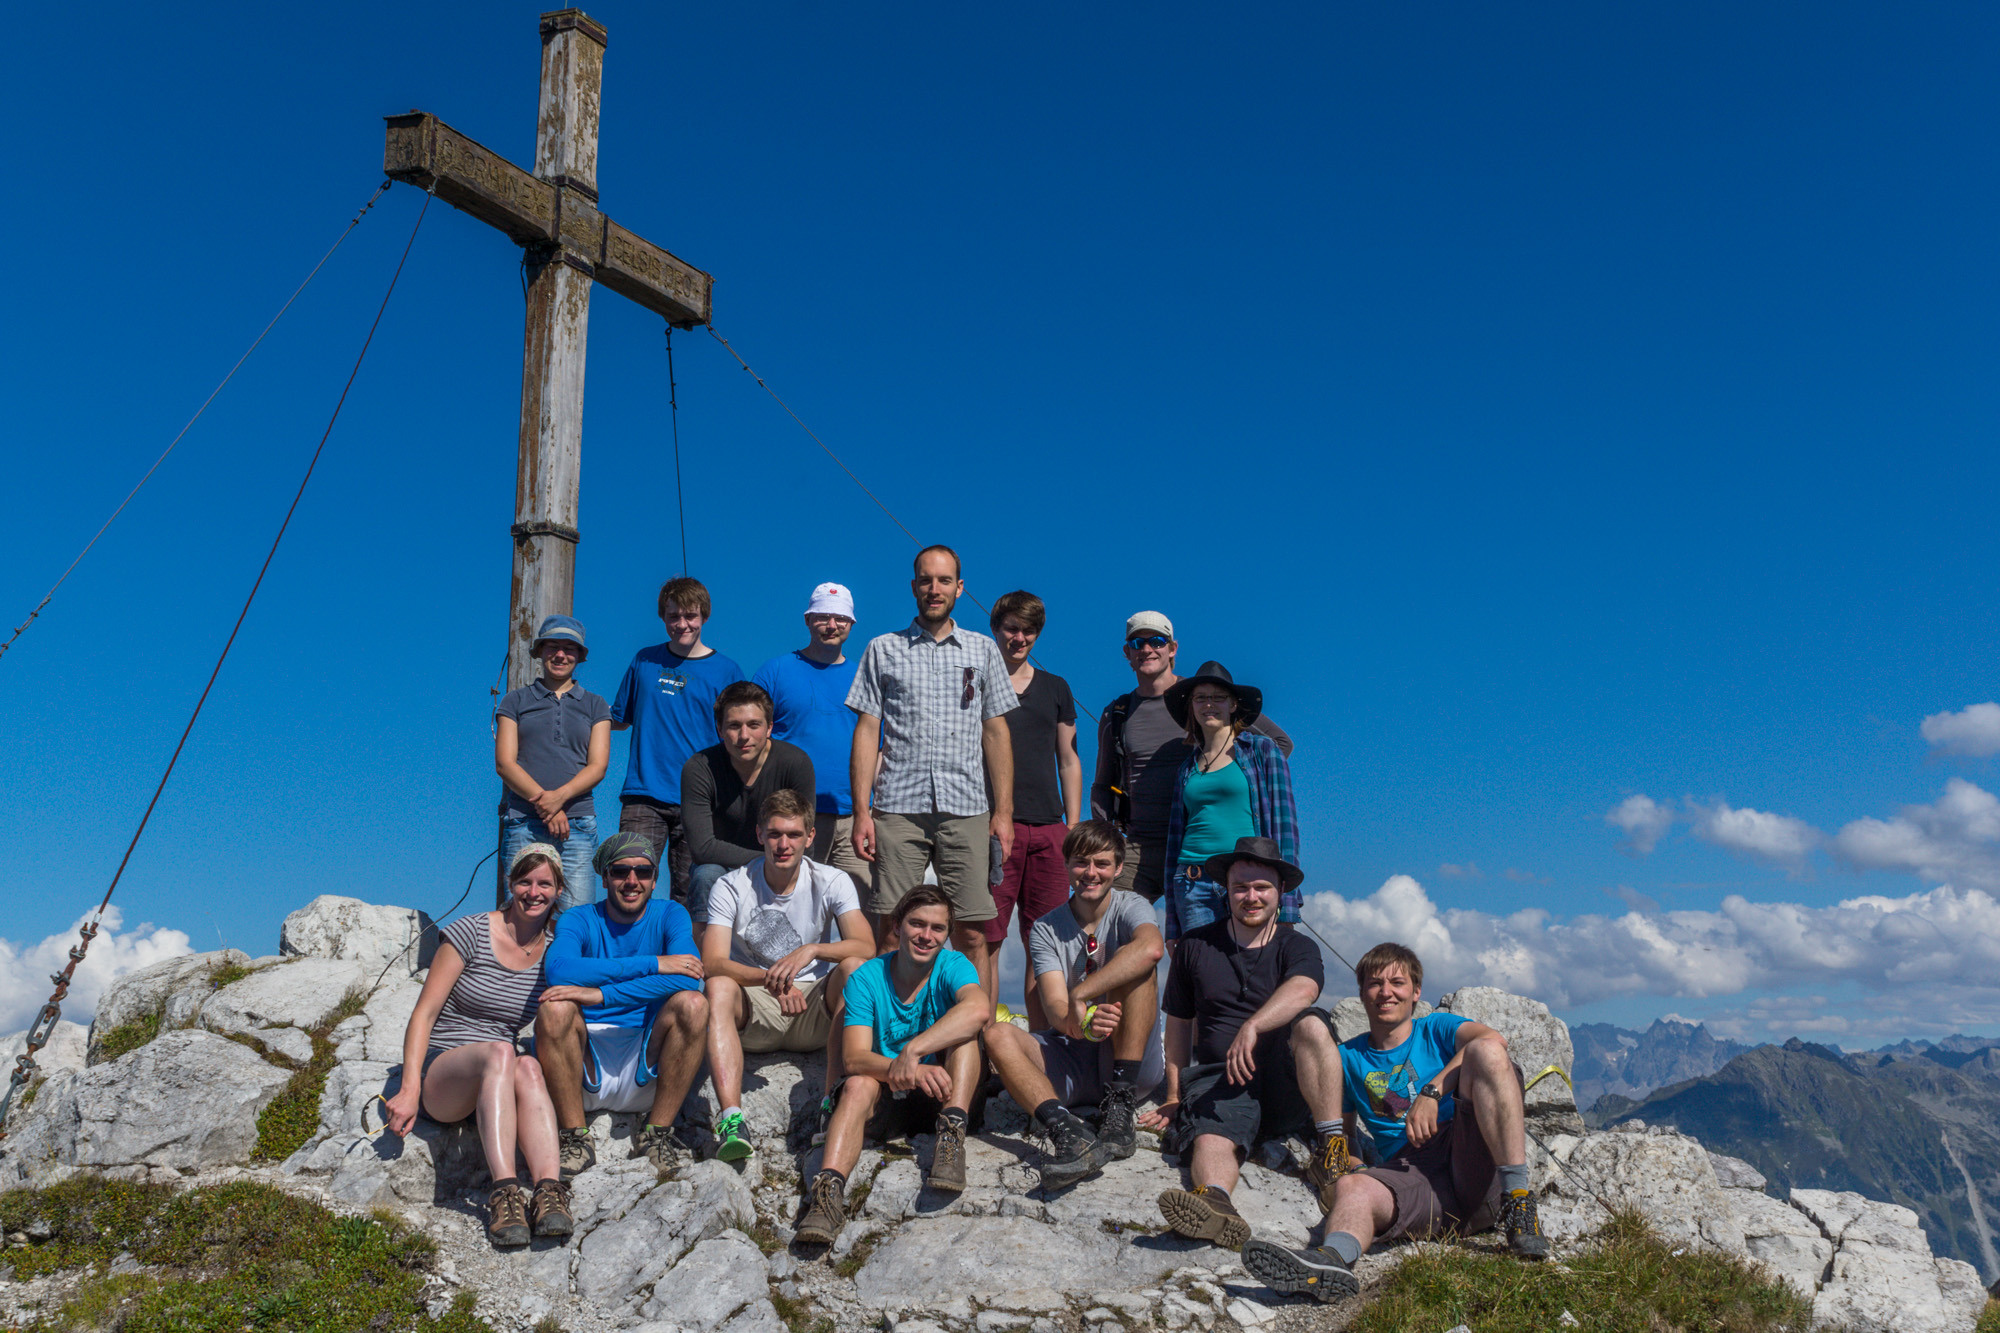
\includegraphics[width=0.45\textwidth]{figs/allgemein/gipfel.jpg}
\caption{Gipfelbild 2013}
\end{figure}

\end{document}
